\subsection{Slučaj upotrebe: Pregled i odobravanje materijala}

\subsubsection*{Kratak opis}

Projektni menadžer pregleda materijale koje su članovi tima predali za svoje zadatke na filmu i odobrava ih ili ih vraća na doradu sa komentarom. Kada se materijal odobri, zadatak kome pripada se smatra završenim.

\subsubsection*{Akteri}
\begin{itemize}
    \item \textbf{Projektni menadžer}: pregleda predate materijale i odlučuje da li se odobravaju.
\end{itemize}

\subsubsection*{Preduslovi}
\begin{itemize}
    \item Projektni menadžer je prijavljen na sistem.
    \item Film postoji u sistemu (slučaj upotrebe ,,Kreiranje filmskog projekta'').
\end{itemize}

\subsubsection*{Postuslovi}
\begin{itemize}
    \item Pregledani materijal je u stanju ,,Odobren'' ili ,,Vraćen na doradu''.
    \item Stanje zadatka kome materijal pripada je ažurirano.
    \item Član tima koji je predao materijal je obavešten o odluci.
\end{itemize}

\subsubsection*{Osnovni tok}
\begin{enumerate}
    \item Projektni menadžer bira film.
    \item Sistem prikazuje materijale tog filma koji čekaju pregled (slučaj upotrebe ,,Predaja materijala'').
    \item Projektni menadžer bira materijal.
    \item Sistem prebacuje materijal u stanje ,,U pregledu'' i prikazuje ga, zajedno sa zadatkom kome pripada i ranije predatim verzijama sa komentarima.
    \item Projektni menadžer pregleda materijal i odobrava ga.
    \item Sistem prebacuje materijal u stanje ,,Odobren'', a zadatak u stanje ,,Završen''.
    \item Sistem obaveštava člana tima koji je predao materijal.
    \item Sistem prikazuje ažuriran spisak materijala koji čekaju pregled.
\end{enumerate}

Koraci 3 do 8 se ponavljaju dok projektni menadžer želi da pregleda još materijala.

\subsubsection*{Podtokovi: /}

\subsubsection*{Alternativni tokovi}

\paragraph*{A1: Nema materijala za pregled}
\begin{itemize}
    \item U koraku 2 osnovnog toka, ako za film nema predatih materijala, sistem o tome obaveštava projektnog menadžera i slučaj upotrebe se završava.
\end{itemize}

\paragraph*{A2: Vraćanje materijala na doradu}
\begin{itemize}
    \item U koraku 5 osnovnog toka, ako materijal nije dobar, projektni menadžer unosi komentar i bira opciju ,,Vrati na doradu'' (slučaj upotrebe ,,Vraćanje materijala na doradu'').
    \item Ako komentar nije unet, sistem traži da se unese i ne nastavlja dalje.
    \item Sistem prebacuje materijal u stanje ,,Vraćen na doradu'', a zadatak u stanje ,,Za Doradu''. Nastavlja se korak 7 osnovnog toka.
\end{itemize}

\paragraph*{A3: Materijal ne može da se otvori}
\begin{itemize}
    \item U koraku 4 osnovnog toka, ako fajl materijala ne može da se otvori, sistem prikazuje grešku.
    \item Projektni menadžer vraća materijal na doradu sa komentarom da fajl nije ispravan. Nastavlja se drugi korak alternativnog toka A2.
\end{itemize}

\subsubsection*{Specijalni zahtevi}
\begin{itemize}
    \item Materijale filma može da odobrava samo projektni menadžer tog filma.
    \item Sistem čuva sve predate verzije materijala i sve odluke o njima.
\end{itemize}

\subsubsection*{Dodatne informacije}
\begin{itemize}
    \item Materijal može biti storyboard, dizajn lika ili okruženja, animacija, zvuk ili montirana sekvenca.
    \item Stanja materijala: ,,Predat'', ,,U pregledu'', ,,Odobren'' i ,,Vraćen na doradu''.
    \item Komentar pri vraćanju na doradu (alternativni tok A2) je obavezan.
\end{itemize}

\begin{figure}[H]
	\centering
	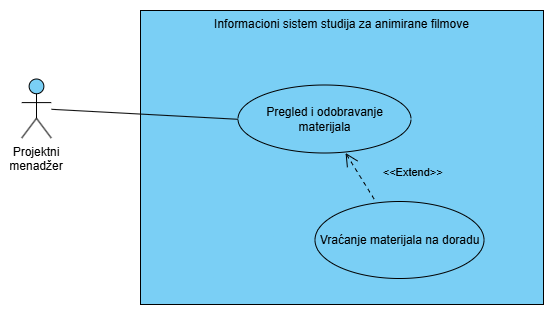
\includegraphics[width=\textwidth]{./dijagrami/dijagrami_slucajeva_upotrebe/pregled_i_odobravanje_materijala.png}
	\caption{Dijagram slučaja upotrebe ,,Pregled i odobravanje materijala''}
 \end{figure}

\begin{figure}[H]
	\centering
	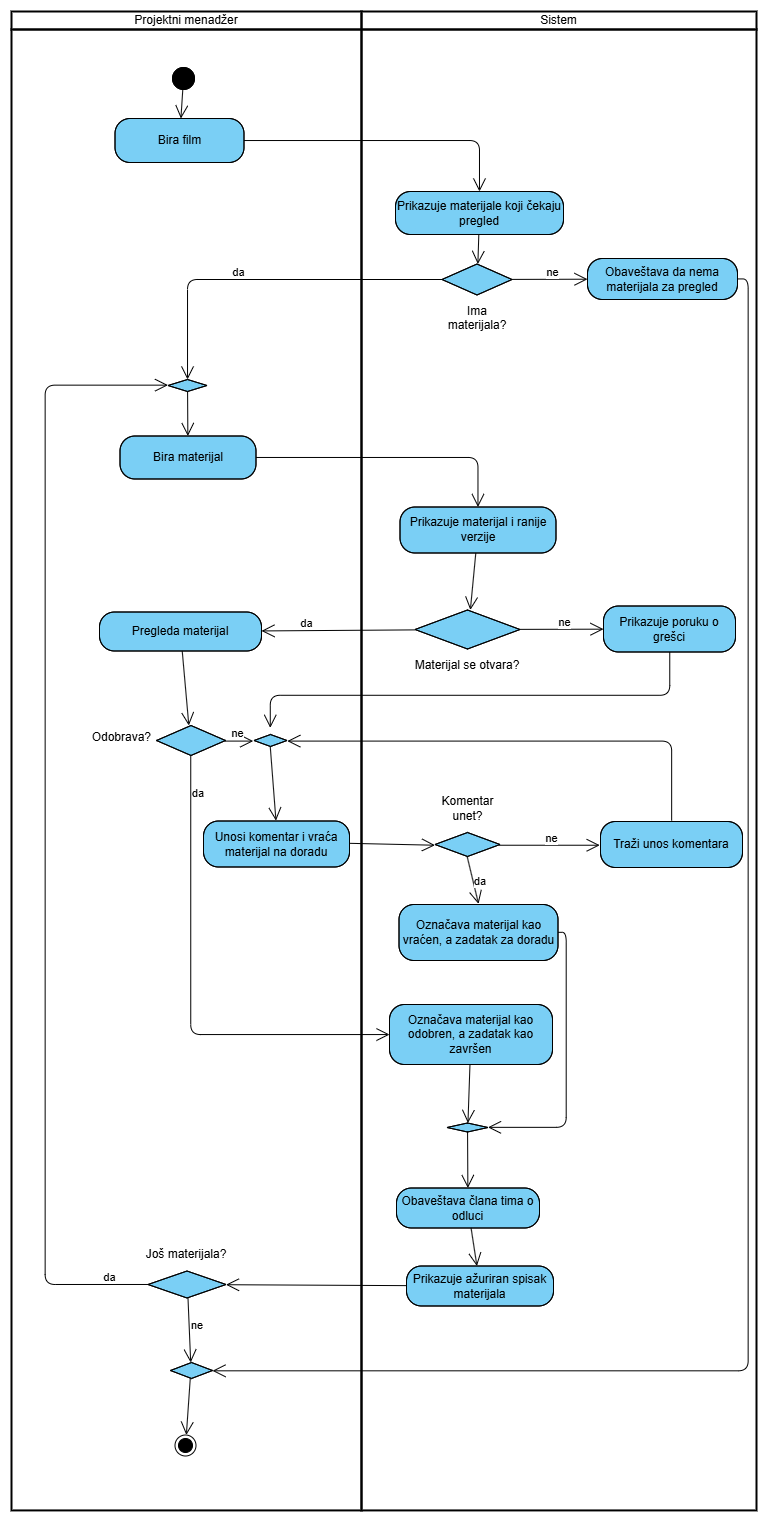
\includegraphics[width=\textwidth,height=0.85\textheight,keepaspectratio]{./dijagrami/dijagrami_aktivnosti/pregled_i_odobravanje_materijala.png}
	\caption{Dijagram aktivnosti ,,Pregled i odobravanje materijala''}
 \end{figure}

\begin{figure}[H]
	\centering
	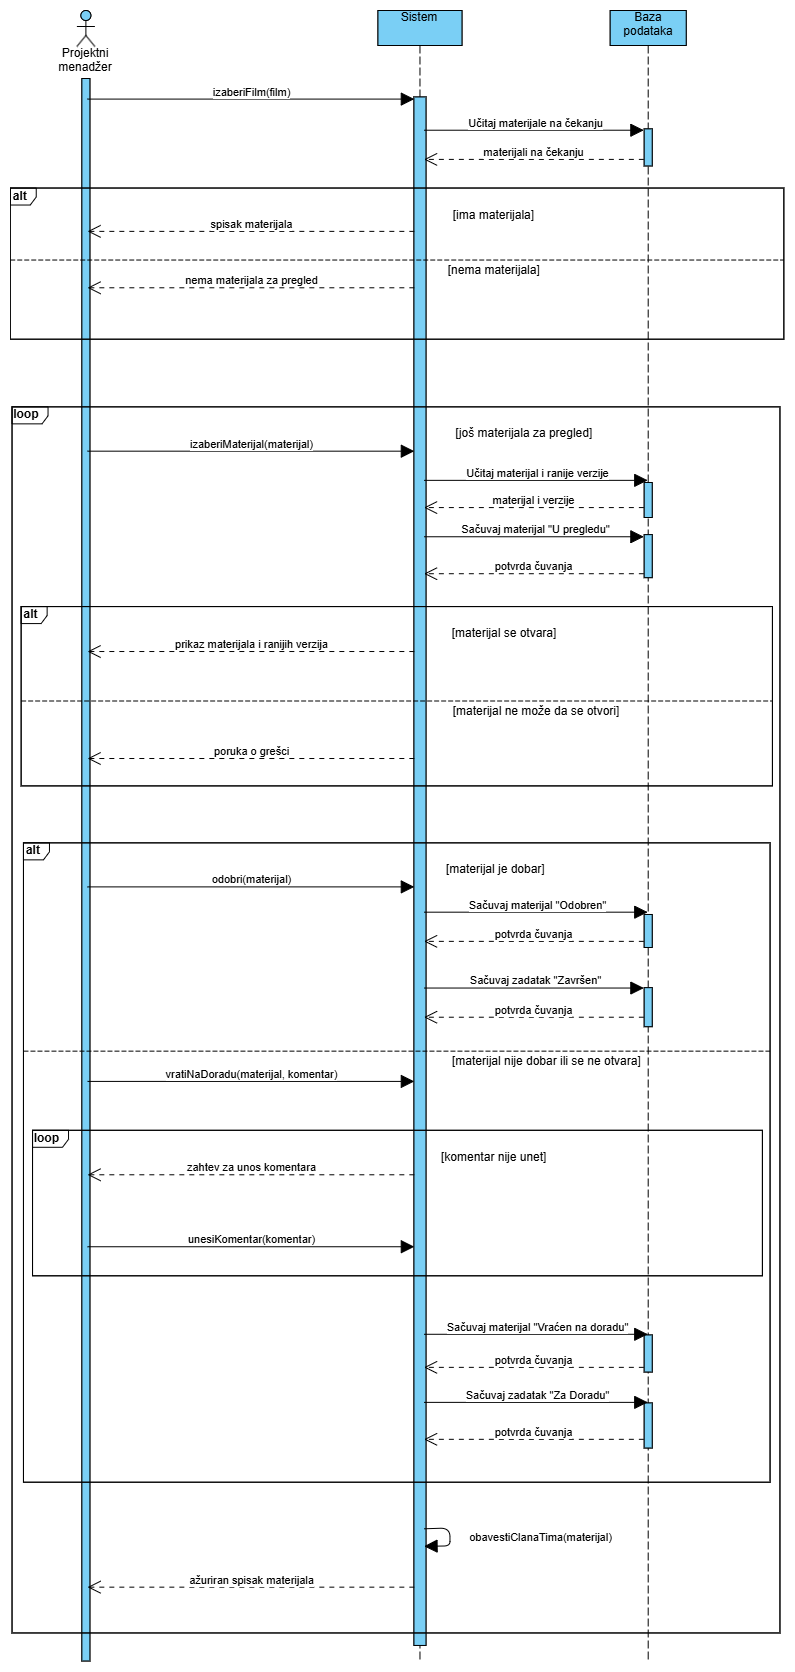
\includegraphics[width=\textwidth,height=0.9\textheight,keepaspectratio]{./dijagrami/dijagrami_sekvence/pregled_i_odobravanje_materijala.png}
	\caption{Dijagram sekvence ,,Pregled i odobravanje materijala''}
 \end{figure}

\begin{figure}[H]
	\centering
	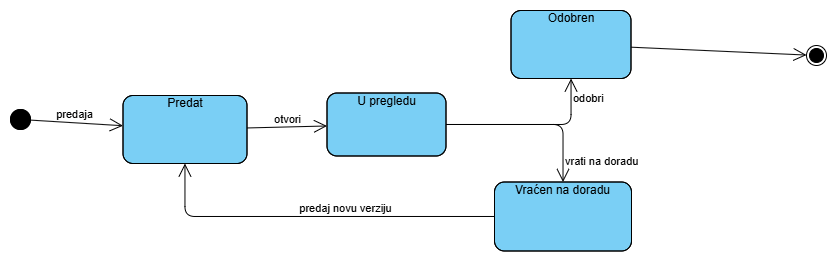
\includegraphics[width=\textwidth]{./dijagrami/dijagrami_stanja/pregled_i_odobravanje_materijala.png}
	\caption{Dijagram stanja materijala}
 \end{figure}

\newpage
